\documentclass{article}
\usepackage[UTF8]{ctex}
\usepackage[tc]{titlepic}
\usepackage{titlesec}
\usepackage{cite}
\usepackage{fancyhdr}
\usepackage{booktabs}
\usepackage{graphicx}
\usepackage{geometry}
\usepackage[section]{placeins}
\usepackage{amsmath}
\usepackage{algorithm}
\usepackage{algorithmic}
\usepackage{float}
\usepackage{amsfonts}
\usepackage{subcaption}
\usepackage[version=4]{mhchem}
\usepackage{siunitx}
\geometry{a4paper,scale=0.8}
\pagestyle{fancy}

\lhead{Final Project\\\today}
\chead{中国科学技术大学\\数学建模课程}

\rhead{Final project\\ {\CTEXoptions[today=old]\today}}
\newcommand{\upcite}[1]{\textsuperscript{\cite{#1}}}

\titleformat*{\section}{\bfseries\Large}
\titleformat*{\subsection}{\bfseries\large}

\title{\bfseries 锂电池晶枝生长的蒙特卡洛模拟}

\author{
 刘行 \quad PB22000150\\
    \and
 贺修凝 \quad PB22000120     
}
\begin{document}
\maketitle
\begin{abstract}
锂离子电池因其高能量密度被广泛应用于电子设备和电动汽车,但充放电过程中锂金属负极表面易形成树枝状枝晶,导致电池短路、过热甚至起火等安全隐患。枝晶生长是一个受锂离子扩散、电场分布及固体电解质界面膜(SEI)特性共同影响的复杂随机过程。本文基于扩散限制聚集(DLA)模型,通过蒙特卡洛方法完成了锂枝晶生长的二维和三维模拟,在传统随机扩散模型的基础上,创新性地耦合了SEI膜动态演化和电场分布的影响。\\

\textbf{关键词:} 锂离子电池;锂枝晶;蒙特卡洛模拟;扩散限制聚集(DLA);SEI膜;电场耦合 
\end{abstract}


\section{前言}
由于锂离子电池具有能量密度高、循环寿命长、自放电少、可快速充放电及无记忆效应等优点,现已被广泛应用于便携式电子设备(如笔记本电脑、平板电脑和手机等)、航空航天、电动汽车等领域。2019年10月9日,瑞典皇家科学院宣布,将2019年若贝尔化学奖授予约翰.古迪纳夫、斯坦利.惠廷厄姆和吉野彰,以表彰他们在锂离子电池研发领域做出的卓越贡献。\\

然而,在电池的使用过程中,长时间的充放电循环,特别是快速充电过程中,锂离子嵌入负极时,由于电荷的不均匀分布导致金属锂沿着晶面取向沉积,放电过程中这部分锂不能及时溶解,累积形成锂枝晶(图1),
\begin{figure}[H]
 \centering
 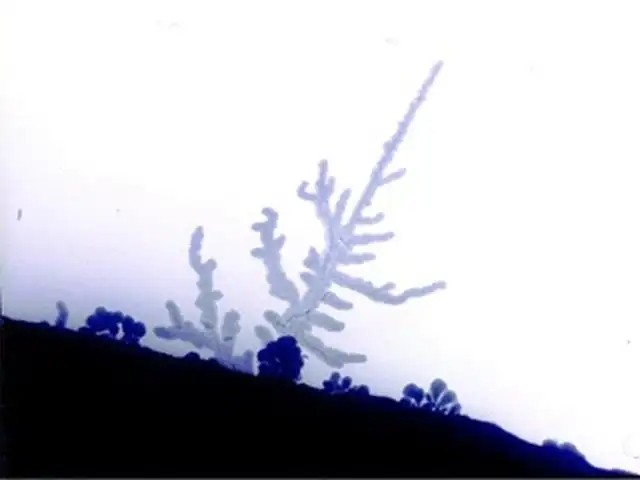
\includegraphics[scale=0.45]{figs/2.jpg}
\caption{典型的树枝状锂枝晶的形貌$^{\textup{\cite{ref1}}}$}
\end{figure}

\noindent 轻则引起锂离子电池的性能衰退,重则引发电池短路(图2)、爆炸、甚至火灾$^{\textup{\cite{ref2,ref3}}}$。因此,理解和预测枝晶
的生长行为对于锂电池的安全性和循环寿命至关重要。枝晶生长是一个复杂的随机过程,受到多种因素如锂离子扩散、电场分布、SEI膜特性的影响,已经很难用传统的宏观模型来精确描述其微观形成机制。\\
\begin{figure}[H]
 \centering
 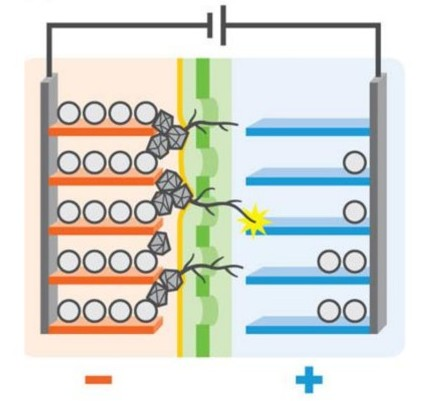
\includegraphics[scale=0.8]{figs/3.jpg}
\caption{锂枝晶的生成可能刺破隔膜,引起短路(图片来源:Sutori)}
\end{figure}
扩散限制凝聚Diffusion-limited Aggregation(DLA)模型是一种描述粒子随机行走并聚集形成分型结构的模型。将锂电池中枝晶的生长过程抽象为电极表面的粒子沉积问题,并利用DLA模型进行模拟。在锂电池枝晶生长中,可以类比为电解液中的锂离子(\ce{Li+})随机扩散到电极表面,并在电场作用下“附着”到正在生长的枝晶上,从而使枝晶不断延伸和分支。


\section{相关工作}
\subsection{锂电池化学反应原理}
\begin{figure}[H]
 \centering
 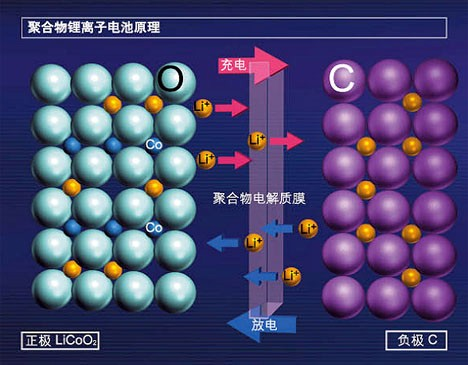
\includegraphics[scale=0.6]{figs/1.jpg}
\caption{锂离子电池原理图(图片来源:百度百科)}
\end{figure}

	锂离子电池充电时会发生如下化学反应:
		\begin{itemize}
			\item 阳极: \ce{LiCoO2 -> CoO2 + Li+ + e-}
			\item 阴极: 石墨\ce{ + Li+ + e- -> LiC6}, 副反应 \ce{Li + e- -> Li v}
		\end{itemize}
		
其中的\ce{Li v}就是锂枝晶的来源。

\subsection{锂枝晶生长的机制}

锂枝晶的形成可划分为三个阶段,具体过程如下: 
\begin{itemize}
\item \textbf{第一阶段:成膜阶段} \\ 
在充放电过程中,锂金属负极因高活泼性与电解液反应,生成固体电解质界面膜(SEI膜)。该膜作为隔离电解液与金属锂的介质,虽能阻止二者持续反应,但允许部分Li$^{+}$透过并在电极表面沉积。  

\item \textbf{第二阶段:成核阶段} \\ 
随着沉积过程推进,锂离子被还原为锂原子,后者逐渐聚集形成微小晶核。随后,锂离子在负极表面发生不均匀沉积,产生不规则凸起,最终顶破原始SEI膜。  

\item \textbf{第三阶段:生长阶段} \\ 
在特定动力学条件下,锂沉积表现出明显的各向异性——沿长度方向的生长速率显著快于径向,促使枝晶状结构逐步形成并延伸。 
\end{itemize} 
\begin{figure}[H]
 \centering
 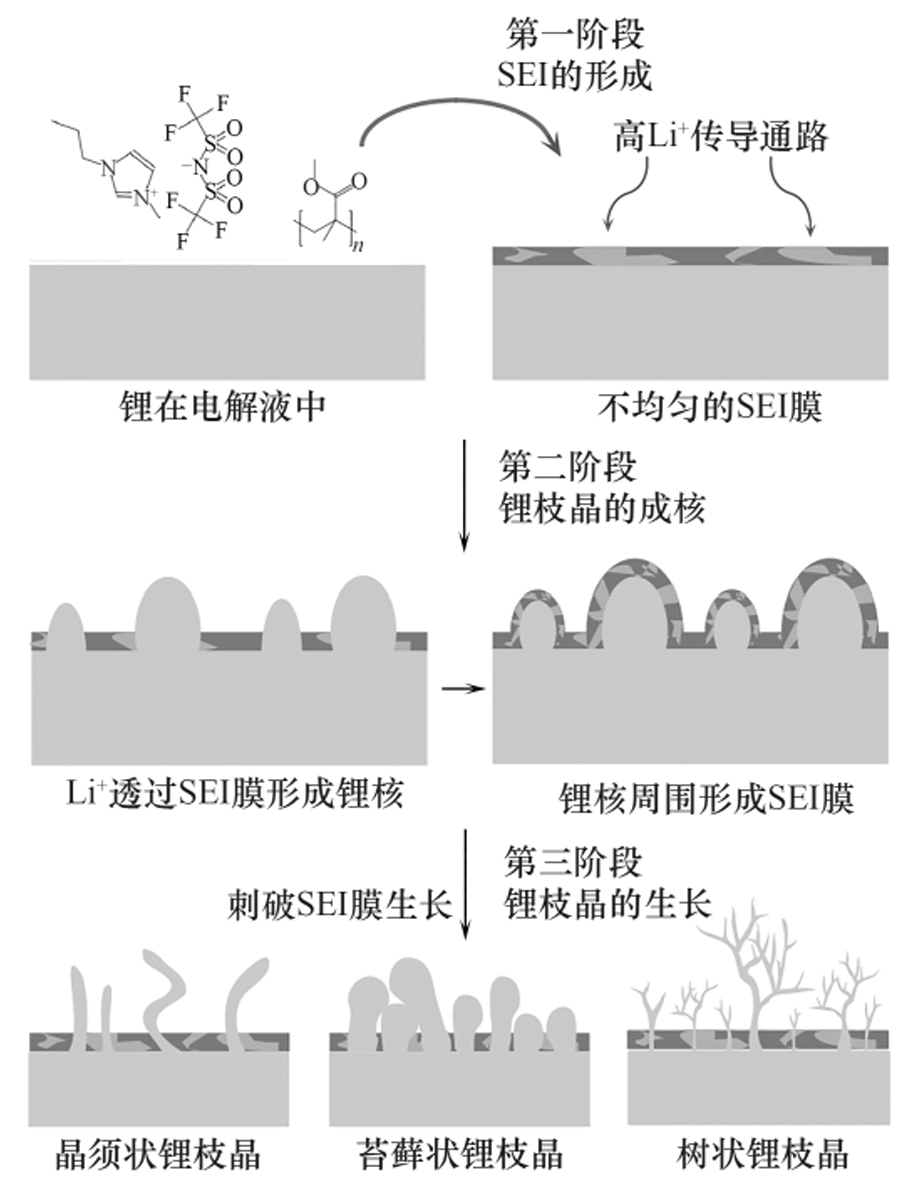
\includegraphics[scale=0.7]{figs/4.png}
\caption{ 枝晶的生长过程示意图$^{\textup{\cite{ref11}}}$}
\end{figure}

\subsection{扩散限制凝聚(Diffusion-limited Aggregation, DLA)模型}
DLA模型由Witten和Sander于1981年提出,用于描述粒子通过随机扩散形成分形结构的动力学过程$^{\textup{\cite{ref4}}}$。其基本算法可表述为:
\begin{algorithm}[H]
\caption{DLA模拟流程}
\begin{algorithmic}[1]
\STATE 初始化:在二维/三维空间中心设置种子粒子
\FOR{每个新粒子}
    \STATE 从边界随机释放粒子
    \WHILE{粒子未附着}
        \STATE 执行随机行走:$x_{t+1} = x_t + \Delta r$, $\Delta r \sim \mathcal{N}(0,2D\Delta t)$
        \IF{接触已有团簇}
            \STATE 永久附着并成为新团簇部分
        \ENDIF
    \ENDWHILE
\ENDFOR
\end{algorithmic}
\end{algorithm}

其中$D$为扩散系数,$\Delta t$为时间步长。\\


\section{问题分析}
\subsection{锂离子在液态电解液中的存在形式}
		锂离子在非水电解液中几乎总是以溶剂化形式存在, 可记作 \ce{Li+(S)_n} 复合物, 其中溶剂分子 (如碳酸酯的羰基氧, 醚氧等) 配位于 \ce{Li+} 周围.

		例如, 在 $\SI{1}{mol/L}$ \ce{LiPF6} /EC-DMC 电解液中, \ce{Li+} 的第一溶剂壳配位数通常为 $4 \sim 6$, 具体取决于溶剂比例 $^\textup{\cite{ref5}}$. 模拟与实验表明 ,\ce{Li+} 优选形成四面体配位结构 (配位数约为 $4$). 不同溶剂结构对配位能力的影响显著: 线性碳酸酯 (如 EMC) 提供较弱溶剂化, 对应更高的扩散系数, 而环状碳酸酯 (如 EC) 则溶剂化更强 $^\textup{\cite{ref6}}$.

		\ce{Li+} 也可能与 \ce{PF6-} 等阴离子形成接触离子对或更大离子簇. 在含水电解液中, \ce{Li+} 为水合离子, 配位数通常为 $4$. 在高浓度或无溶剂体系 (如聚电解质或离子液体) 中, 阴离子参与配位, 形成溶剂隔离离子对或多离子络合物$^\textup{\cite{ref5, ref7}}$.

	\subsection{粒子随机运动机制与扩散:估算平均自由程}
		在无外场条件下, \ce{Li+} 通过热运动 (布朗运动) 扩散, 其扩散系数 $D$ 可由 Stokes-Einstein 关系近似估算:
		\begin{equation}
		D \approx \frac{k_{B} T}{6 \pi \eta r}
		\end{equation}
		其中, $r$ 为溶剂化离子半径, $\eta$ 为溶剂粘度. 典型碳酸酯电解液中, $\eta \approx 10^{-3}\,\si{Pa\cdot s}$, $r \approx 0.2 \sim \SI{0.3}{nm}$, 可得 $D \approx 10^{-10} \sim 10^{-9}\,\si{m^{2}/s}$.

		实验测量 (如旋转圆盘电极与 PFG-NMR) 亦支持此量级. 例如, 在 $\SI{1}{mol/L}$ \ce{LiPF6} /EC-DMC 中, \ce{Li+} 的 $D$ 可达 $1.4 \times 10^{-9}\,\si{m^{2}/s}$ $^\textup{\cite{ref8}}$, 其中直链溶剂 (EMC) 下略高于环状溶剂 (EC) $^\textup{\cite{ref6}}$. PFG-NMR研究也发现 $D_{\ce{Li+}}$ 约为 $10^{-10} \sim 10^{-9}\,\si{m^{2}/s}^\textup{\cite{ref9}}$
		
 
 	估算\textbf{平均自由程}可将扩散过程视为高频碰撞: \ce{Li+} 的热速度可估为
 		\begin{equation}
 		v_{\mathrm{th}} \sim \sqrt{\frac{3 k_{B} T}{m}}
 		\end{equation}
 		其中 $m$ 包括溶剂化团簇质量. 在 $T = \SI{300}{K}$ 下, $v_{\mathrm{th}} \approx 10^{2} \sim 10^{3}\,\si{m/s}$. 其平均自由程为:
 		\begin{equation}
 		l \approx \frac{3D}{v_{\mathrm{th}}}
 		\end{equation}
 		约为 $10^{-11} \sim 10^{-10}\,\si{m}$, 相当于几埃, 与液体分子间距相当$^\textup{\cite{ref7}}$.


	\subsection{电场作用下的定向迁移}
		在电场 $\mathbf{E}$ 作用下, \ce{Li+} 获得漂移速度 $v_{d}$:
		\begin{equation}
		v_{d} = \mu E
		\end{equation}
		其中迁移率 $\mu$ 可由爱因斯坦关系给出:
		\begin{equation}
		\mu = \frac{Dq}{k_{B} T}
		\end{equation}
		例如, $D = 1 \times 10^{-9}\,\si{m^{2}/s}$, $T=\SI{300}{K}$, 得 $\mu \approx 4 \times 10^{-8}\,\si{m^{2}/(V\cdot s)}$, 对应在 $E = 10^{4}\,\si{V/m}$ 下的漂移速度为 $v_{d} \approx 4 \times 10^{-4}\,\si{m/s}$.

		扩散在 $t=\SI{1}{s}$ 内的均方根位移:
		\begin{equation}
		\sqrt{2Dt} \approx 4.5 \times 10^{-5}\,\si{m}
		\end{equation}
		即``扩散速度''量级约 $10^{-4}\,\si{m/s}$, 说明在中等电场下漂移速度与扩散速度可为同一数量级 (弱场时扩散占优, 强场时漂移主导). 文献指出, 溶剂种类影响扩散: 例如直链碳酸酯 (EMC) 中 \ce{Li+} 扩散略大于环状碳酸酯 (EC) $^\textup{\cite{ref6}}$. 当 $qE$ 显著超过$k_BT$时, \ce{Li+} 几乎沿电场线定向迁移; 反之若$k_BT\gg qE$, 分布趋于各向同性 $^\textup{\cite{ref10}}$.

		在 DLA 模拟中, 我们引入偏置的随机行走模型来模拟电场下的定向迁移 $^\textup{\cite{ref10}}$:
		\begin{equation}
		P_{move}(\Delta \mathbf{r}) \propto \exp\left( \frac{q \mathbf{E} \cdot \Delta \mathbf{r}}{k_{B} T} \right)
		\end{equation}

		\noindent 从而在统计上偏置粒子沿电场移动. 
\section{模型的假设}
基于DLA框架的锂枝晶生长模拟采用以下基本假设:

\begin{enumerate}
    \item \textbf{三因素主导假设}:
    \begin{itemize}
        \item 仅考虑电场作用、锂离子自由扩散和SEI膜影响,忽略其他次要因素(如温度波动、电解液对流、机械应力等)
        \item 假设电解液浓度恒定,不考虑充放电过程中局部浓度变化
    \end{itemize}


    \item \textbf{电场准静态假设}:
    \begin{itemize}
        \item 外电场在模拟时间尺度内保持稳定,忽略电极极化导致的场强变化
        \item 空间电场分布仅由宏观电极几何决定,不考虑微观枝晶对电场的反馈作用
    \end{itemize}

    \item \textbf{粒子独立性假设}:
    \begin{itemize}
        \item 锂离子在扩散过程中无电相互作用(忽略离子-离子关联效应)
        \item 附着概率仅取决于局部条件,与历史路径无关(马尔可夫过程)
    \end{itemize}

    \item \textbf{基底理想化假设}:
    \begin{itemize}
        \item 平行板电极表面为完美光滑平面,忽略实际电极的粗糙度与缺陷
        \item 忽略点电极的体积,视为一个完美的点

    \end{itemize}
\end{enumerate}

\section{符号说明}
\begin{table}[H]
\centering
\caption{模型主要符号与物理意义}
\begin{tabular}{ccc}
\toprule
\textbf{符号} & \textbf{物理意义} & \textbf{单位} \\
\midrule
$D$ & 锂离子扩散系数 & \si{m^2/s} \\
$\mathbf{E}$ & 外加电场强度 & \si{V/m} \\
$k_B$ & 玻尔兹曼常数 & \si{J/K} \\
$T$ & 绝对温度 & \si{K} \\
$\eta$ & 电解液粘度 & \si{Pa\cdot s} \\
$r$ & 溶剂化锂离子半径 & \si{nm} \\
$\mu$ & 锂离子迁移率 & \si{m^2/(V\cdot s)} \\
$v_{th} $& 锂离子热速度 & \si{m/s}\\
$v_d$ & 锂离子漂移速度 & \si{m/s} \\
$l $&锂离子平均自由程& \si{m}\\
$q$ & 锂离子电荷量 & \si{C} \\
$\Delta t$ & 模拟时间步长 & \si{s} \\
$\Delta r$ & 随机行走步长 & \si{m} \\
$P_{\text{attach}}$ & 粒子附着概率 & 无量纲 \\
$P_{\text{move}}$ & 粒子移动概率 & 无量纲 \\
\bottomrule
\end{tabular}
\label{tab:symbols}
\end{table}
\section{数学模型建立}
\subsection{二维模型构建}
基于扩散限制聚集(DLA)框架,建立锂枝晶生长的二维随机模型:
\subsubsection{随机行走模型}
电场影响的\ce{Li+}在溶剂中随机行走概率模型为:
\begin{equation}
P_{\text{move}}(x,y \to x',y') = \frac{\exp\left(\beta \mathbf{E}(x,y) \cdot \Delta\mathbf{r}\right)}{\sum\limits_{\Delta\mathbf{r}\in \mathcal{N}_4}\exp\left(\beta \mathbf{E}(x,y) \cdot \Delta\mathbf{r}\right)}
\end{equation}

其中:
\begin{itemize}
\item $\beta=(k_B T)^{-1}$ 
\item $\Delta r$是随机行走步长,这里取\ce{Li+}的平均自由程$l=10^{-10}\,\si{m}$ 
\item $\mathcal{N}_4$为4邻域位移集合$\{(1,0),(0,1),(-1,0),(0,-1)\}$
\end{itemize}
\subsubsection{随机附着模型}
SEI膜影响的附着概率模型为:

\begin{equation}
P_{\text{attach}} = P_0 \cdot \exp\left(-\lambda \sum\limits_{\Delta\mathbf{r}\in \mathcal{N}_8} \text{SEI}\left((x,y)+\Delta r\right)\right)
\end{equation}
其中:
\begin{itemize}
\item $P_0$ 为基准附着概率(无SEI膜时的初始概率)
\item $\lambda$ 为SEI膜对附着概率的影响参数,默认值$\lambda=0.1$
\item $\text{SEI}(x,y)$ 为位置$(x,y)$处的SEI膜厚度
\item $\mathcal{N}_8$为8邻域位移集合$\{(1,0),(0,1),(-1,0),(0,-1),(1,1),(-1,1)(1,-1),(-1,-1)\}$
\end{itemize}

\subsection{三维模型构建}
基于扩散限制聚集(DLA)框架,建立锂枝晶生长的三维随机模型:
\subsubsection{随机行走模型}
电场影响的\ce{Li+}在溶剂中随机行走概率模型为:
\begin{equation}
P_{\text{move}}(x,y,z \to x',y',z') = \frac{\exp\left(\beta \mathbf{E}(x,y,z) \cdot \Delta\mathbf{r}\right)}{\sum\limits_{\Delta\mathbf{r}\in \mathcal{N}_6}\exp\left(\beta \mathbf{E}(x,y,z) \cdot \Delta\mathbf{r}\right)}
\end{equation}

其中:
\begin{itemize}
\item $\beta=(k_B T)^{-1}$ 
\item $\Delta r$是随机行走步长,这里取\ce{Li+}的平均自由程$l=10^{-10}\,\si{m}$ 
\item $\mathcal{N}_6$为6邻域位移集合$\{(1,0,0),(0,1,0),(0,0,1),(-1,0,0),(0,-1,0),(0,0,-1)\}$。
\end{itemize}
\subsubsection{随机附着模型}
SEI膜影响的附着概率模型为:

\begin{equation}
P_{\text{attach}} = P_0 \cdot \exp\left(-\lambda \sum\limits_{\Delta\mathbf{r}\in \mathcal{N}_{26}} \text{SEI}\left((x,y,z)+\Delta r\right)\right)
\end{equation}
其中:
\begin{itemize}
\item $P_0$ 为基准附着概率(无SEI膜时的初始概率)
\item $\lambda$ 为SEI膜对附着概率的影响参数,默认值$\lambda=0.1$
\item $\text{SEI}(x,y,z)$ 为位置$(x,y,z)$处的SEI膜厚度
\item $\mathcal{N}_{26}$ 为26邻域位移集合,包含所有三维立方网格中面、边、顶点方向的单位位移:
\[
\mathcal{N}_{26} = \big\{ (dx, dy, dz) \mid dx, dy, dz \in \{-1, 0, 1\} \big\} \setminus \{(0, 0, 0)\}
\]
\end{itemize}
\subsection{数值实现算法}
核心模拟流程如算法\ref{alg:dla}所示:

\begin{algorithm}[H]
\caption{锂枝晶生长蒙特卡洛模拟}
\begin{algorithmic}[1]
\STATE 初始化网格$G_{L\times L\times L}$,设置种子粒子
\FOR{每个新粒子$n=1\to N_{\text{max}}$}
    \STATE $(x,y,z) \leftarrow \text{SpawnParticle}()$ \COMMENT{按场类型生成}
    \FOR{$t=1\to T_{\text{max}}$}
        \STATE $(x',y',z') \leftarrow \text{BiasedMove}(x,y,z)$ \COMMENT{式(8),(10)加权移动}
        \IF{接触团簇且 $\text{Rand}() < P_{\text{attach}}$}
            \STATE $G[x',y',z'] \leftarrow 1$ \COMMENT{粒子固定}
            \STATE 更新曲率和SEI厚度
            \STATE \textbf{break}
        \ENDIF
        \STATE $(x,y,z) \leftarrow (x',y',z')$
    \ENDFOR
\ENDFOR
\end{algorithmic}
\label{alg:dla}
\end{algorithm}

\subsection{关键参数设置}
3d模型参数默认值:

\begin{table}[H]
\centering
\caption{模拟参数默认值}
\begin{tabular}{lc}
\toprule
\textbf{参数} & \textbf{取值} \\
\midrule
网格尺寸$L$ & 201 \\
电场强度$E_0$ & \SI{0.01}{V/m} \\
SEI生长率$\alpha$ & 0.01 \\
最大SEI厚度$d_{\text{max}}$ & 1.0 \\
SEI膜对附着概率的影响参数$\lambda$ &0.1\\
最大粒子数$N_{max}$ & 2000\\
最大步数$T_{max}$ & 10000\\
基准附着概率$P_0$ & 1\\
\bottomrule
\end{tabular}
\label{tab:params}
\end{table}
其中,电场强度$E_0$在点电极电场中表示距离点电极$10^{-10}\si{m}$处的电场强度为$E_0$
\subsection{交互界面设计}
\begin{figure}[H]
 \centering
 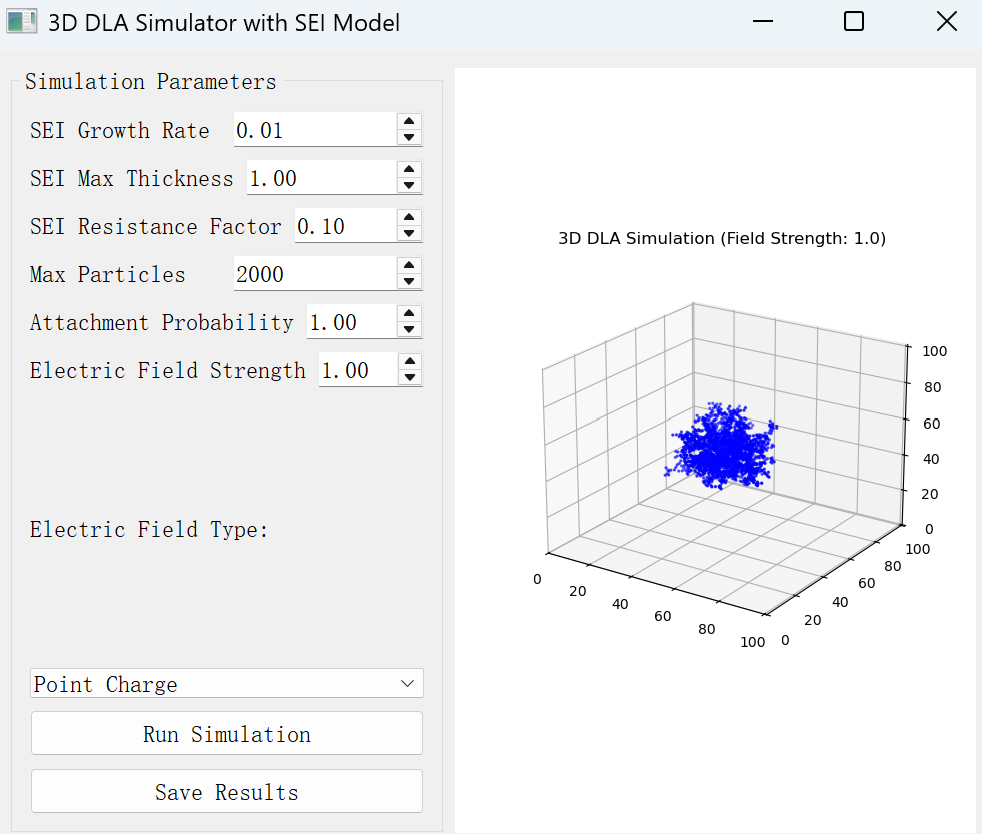
\includegraphics[scale=0.7]{figs/5.png}
\caption{ 交互界面示意图}
\end{figure}

\section{结果(与对比)}
\subsection{模拟结果展示}
\subsubsection{点电极}
\begin{figure}[H]
      \centering
       \begin{minipage}{0.32\textwidth}
                    \centering
                    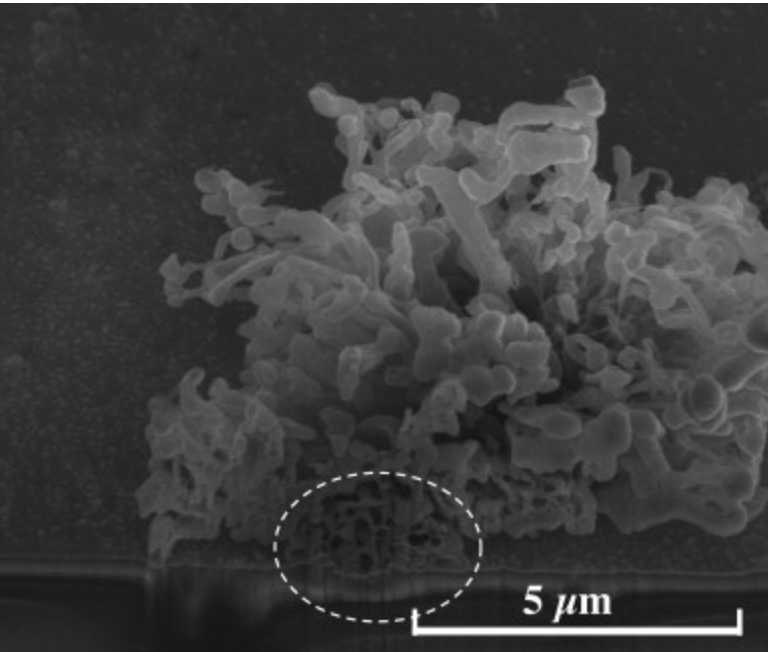
\includegraphics[scale=0.45]{figs/7.png}
                    \caption{点电极锂枝晶显微图$^{\textup{\cite{ref13}}}$}
                   
       \end{minipage}
                \hfill % 添加一些水平空间
                \begin{minipage}{0.32\textwidth}
                    \centering
                    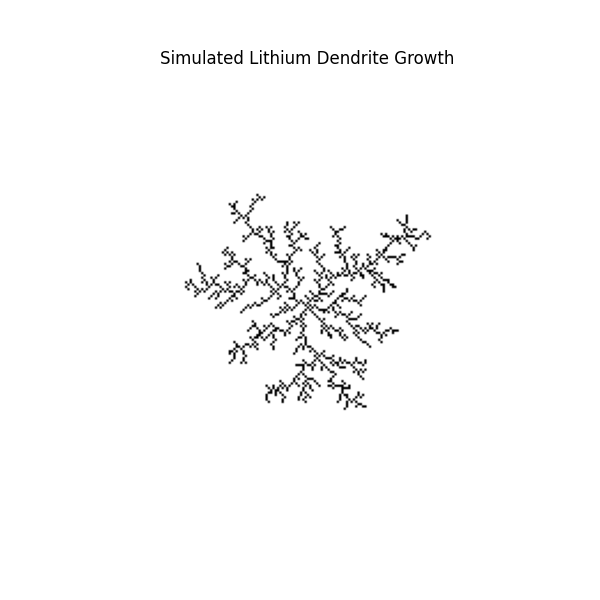
\includegraphics[scale=0.35]{figs/10.png}
                    \caption{点电极锂枝晶二维模拟}
                \end{minipage}
                \hfill % 添加一些水平空间
                \begin{minipage}{0.32\textwidth}
                   \centering
                  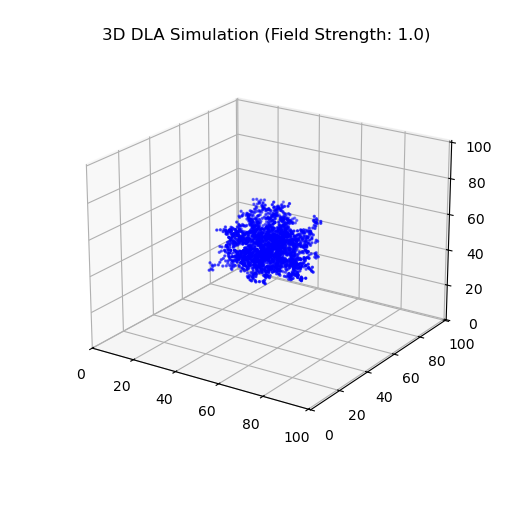
\includegraphics[scale=0.4]{figs/8.png}

                   \caption{点电极锂枝晶三维模拟}
                \end{minipage}
       \end{figure}      
\subsubsection{平行板电极}
\begin{figure}[H]
      \centering
       \begin{minipage}{0.32\textwidth}
                    \centering
                    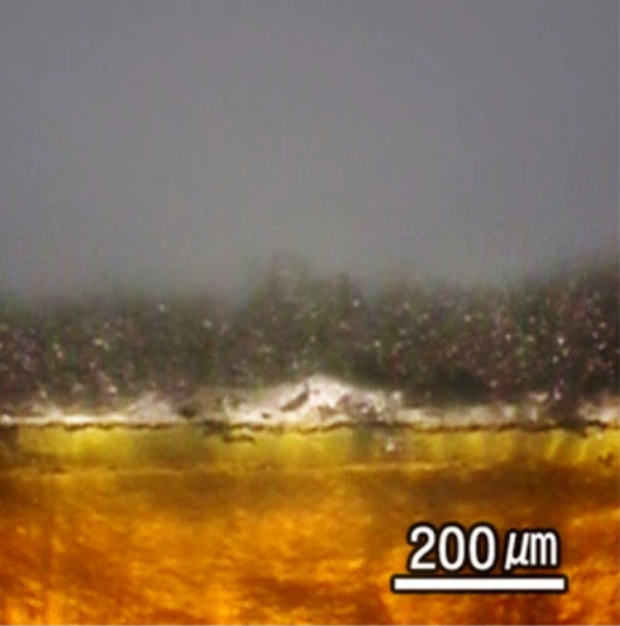
\includegraphics[scale=0.55]{figs/6.png}
                    \caption{平行板电极锂枝晶显微图$^{\textup{\cite{ref12}}}$}
                   
       \end{minipage}
                \hfill % 添加一些水平空间
                \begin{minipage}{0.32\textwidth}
                    \centering
                    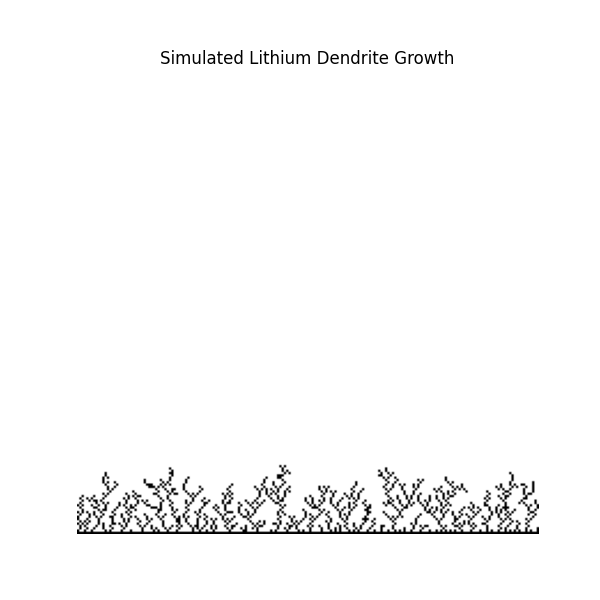
\includegraphics[scale=0.35]{figs/11.png}
                    \caption{平行板电极锂枝晶二维模拟}
                \end{minipage}
                \hfill % 添加一些水平空间
                \begin{minipage}{0.32\textwidth}
                   \centering
                  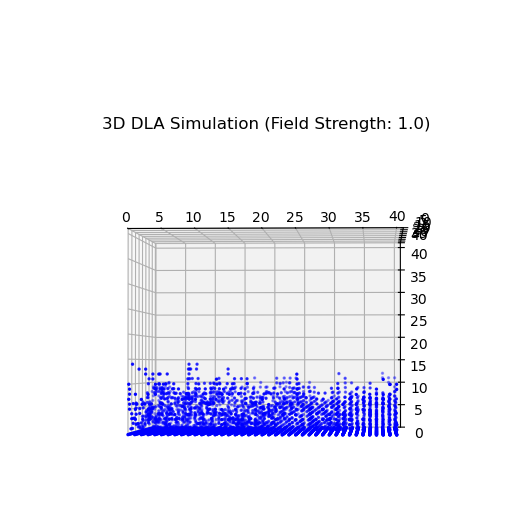
\includegraphics[scale=0.4]{figs/9.png}

                   \caption{平行板电极锂枝晶三维模拟}
                \end{minipage}
       \end{figure}         
 \subsection{枝晶相对填充率分析}
枝晶相对填充率定义为枝晶体积与其延伸范围体积的比值。具体而言,在点电极体系中,该体积范围为由枝晶最远端围绕电极中心所形成的球体体积;在平行板电极体系中,则为由最长枝晶到底面所构成的长方体体积。
\subsubsection{模拟实验}
     \begin{figure}[H]
            \centering
            \begin{minipage}{0.45\textwidth}
\centering
 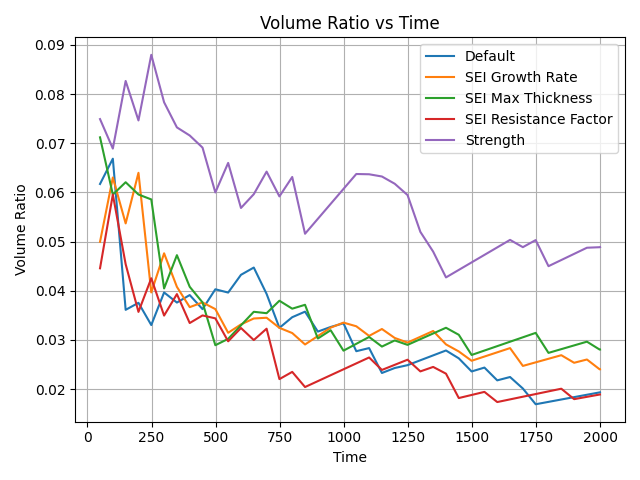
\includegraphics[scale=0.45]{figs/point_volume_ratio_comparison.png}
\caption{不同参数条件下点电极体系中枝晶相对填充率随时间演化。图例表示被提升的默认参数。}
            \end{minipage}
            \hfill % 添加一些水平空间
            \begin{minipage}{0.45\textwidth}
 \centering
 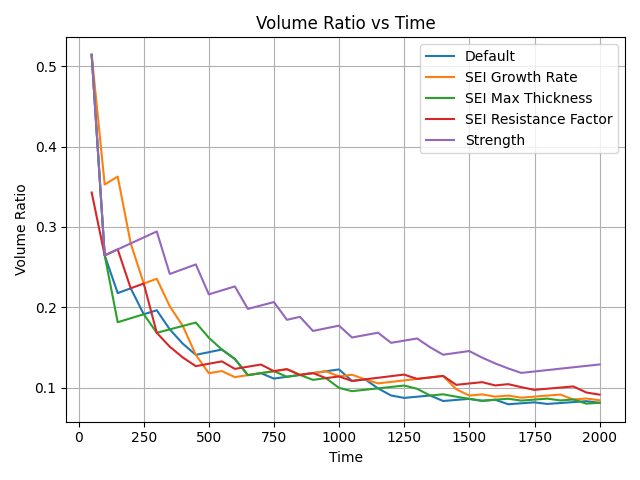
\includegraphics[scale=0.45]{figs/parallel_volume_ratio_comparison.png}
\caption{不同参数条件下平行板电极体系中枝晶相对填充率随时间演化。图例表示被提升的默认参数。}
            \end{minipage}
        \end{figure}
\subsubsection{实验结果分析}
\begin{itemize}
\item 通过对比默认参数与提高SEI生长速率、最大厚度、对附着概率的抑制参数及电场强度的模拟结果,
发现提高电场强度会显著增加枝晶的相对填充率(Volume Ratio),表明电场强度对枝晶生长具有主导作用。
\item 
所有电极体系中枝晶的相对填充率呈现时间依赖性衰减。所有参数组均呈现填充率下降趋势。
\item 
相同电场强度下,点电极体系的枝晶相对填充率远小于平行板电极体系。
\end{itemize}




 \subsection{枝晶分形维数分析}

 分形维数 \( D \) 定义为:
 \[
 D = \lim_{R \to 0} \frac{\log N(R)}{\log R}
 \]
 其中:
 \begin{itemize}
     \item \( R \) 为枝晶簇的最大延伸半径(从中心点到最远粒子的欧氏距离)
     \item \( N(R) \) 为半径 \( R \) 范围内包含的枝晶粒子总数
 \end{itemize}
 
分形维数常常用于量化锂枝晶生长的空间填充特性:
 \begin{itemize}
     \item \( D \approx 1.0 \): 枝晶呈线状生长
     \item \( 1.0 < D < 3.0 \): 分形结构(典型值约2.5-2.8)
     \item \( D \to 3.0 \): 空间完全填充
 \end{itemize}
 \subsubsection{模拟实验}
      \begin{figure}[H]
             \centering
             \begin{minipage}{0.45\textwidth}
 \centering
  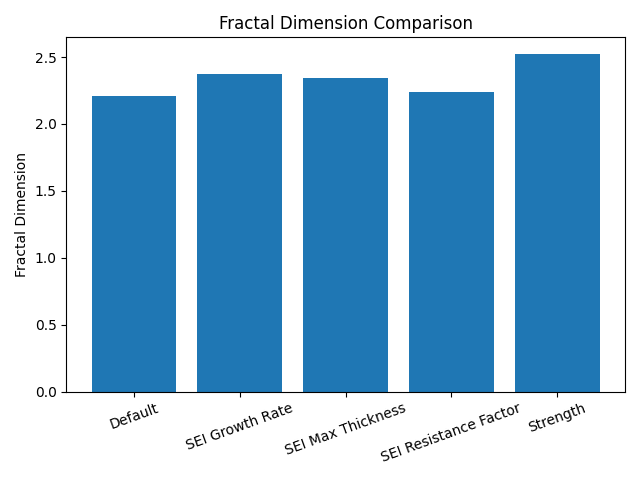
\includegraphics[scale=0.45]{figs/point_fractal_dimension_comparison.png}
 \caption{不同参数条件下点电极体系中枝晶分形维数。图例表示被提升的默认参数。}
             \end{minipage}
             \hfill % 添加一些水平空间
             \begin{minipage}{0.45\textwidth}
  \centering
  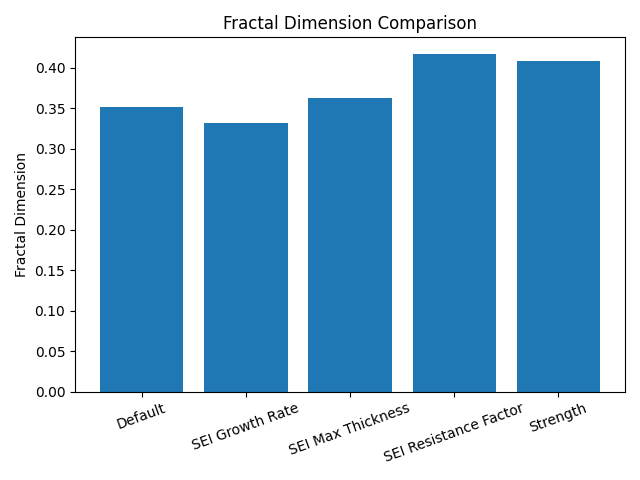
\includegraphics[scale=0.45]{figs/parallel_fractal_dimension_comparison.png}
 \caption{不同参数条件下平行板电极体系中枝晶分形维数。图例表示被提升的默认参数。}
             \end{minipage}
         \end{figure}
\subsubsection{实验结果分析}
 \begin{itemize}
     \item 所有参数组的点电极枝晶的分形维数都在2-2.5之间,呈现典型的分形结构。
     \item 所有参数组的平行板电极枝晶的分形维数都<1.0,呈现线状生长的形态。
 \end{itemize}
  \subsection{枝晶累积生长速度分析}
  累积生长量(Cumulative Growth)是锂枝晶最大延伸距离。时间-累计生长量图的折线斜率表示枝晶的累计生长速度。
        \begin{figure}[H]
               \centering
               \begin{minipage}{0.45\textwidth}
   \centering
    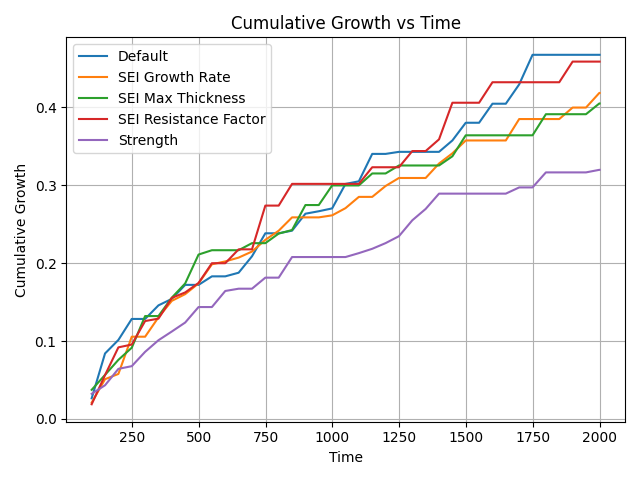
\includegraphics[scale=0.45]{figs/point_cumulative_growth_comparison.png}
   \caption{不同参数条件下点电极体系中枝晶累计生长量随时间演化。图例表示被提升的默认参数。}
               \end{minipage}
               \hfill % 添加一些水平空间
               \begin{minipage}{0.45\textwidth}
    \centering
    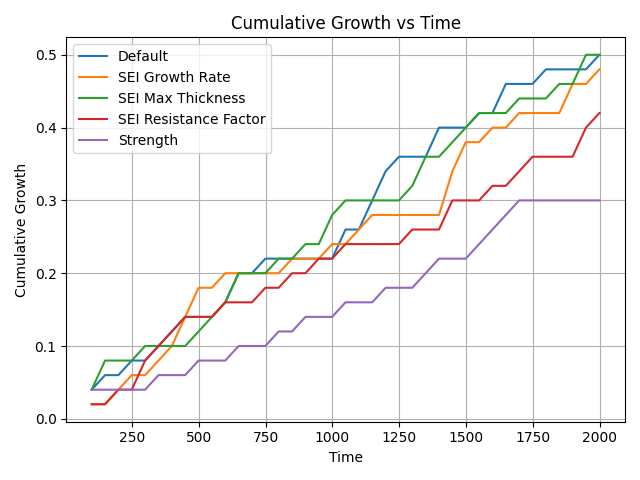
\includegraphics[scale=0.45]{figs/parallel_cumulative_growth_comparison.png}
   \caption{不同参数条件下平行板电极体系中枝晶累计生长量随时间演化。图例表示被提升的默认参数。}
               \end{minipage}
           \end{figure}
  \subsubsection{实验结果分析}
   \begin{itemize}
       \item 通过对比默认参数与提高SEI生长速率、最大厚度、对附着概率的抑制参数及电场强度的模拟结果,
       发现提高电场强度会显著减慢枝晶的累计生长速度,提高SEI生长速率、最大厚度、对附着概率的抑制参数对枝晶累计生长速度也有减缓作用。给抑制枝晶生长提供了参考方法。
       \item 累计生长量每增长一段时间,折线就会出现一个平台,这是枝晶累计生长量的间歇停滞现象。
   \end{itemize}
   
     \subsection{枝晶密度时空规律}
   密度(Density)的定义为每层内枝晶的体积与该层体积的比值。其中,“层” 指的是在空间中,距离底部(如电极底面)或电极中心等参考点具有相同距离范围所划定的区域。
   \subsubsection{模拟实验}

 \begin{figure}[H]
     \centering
     % 第一张图
     \begin{subfigure}[b]{0.19\textwidth}
         \centering
         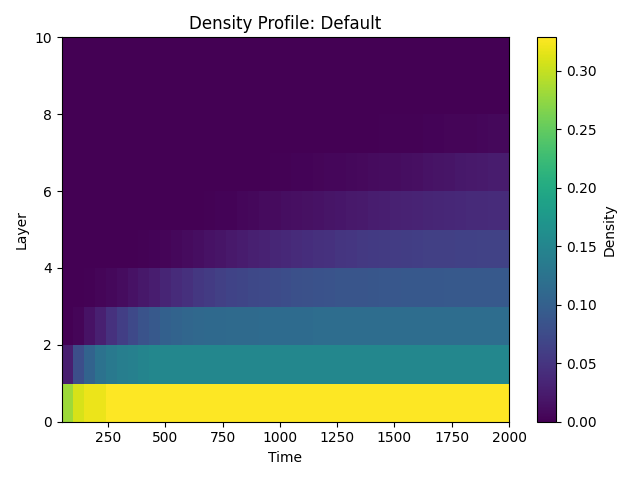
\includegraphics[scale=0.2]{figs/point_density_profile_default.png}
         \caption{默认参数值}
        
     \end{subfigure}
     \hfill
     % 第二张图
     \begin{subfigure}[b]{0.19\textwidth}
         \centering
         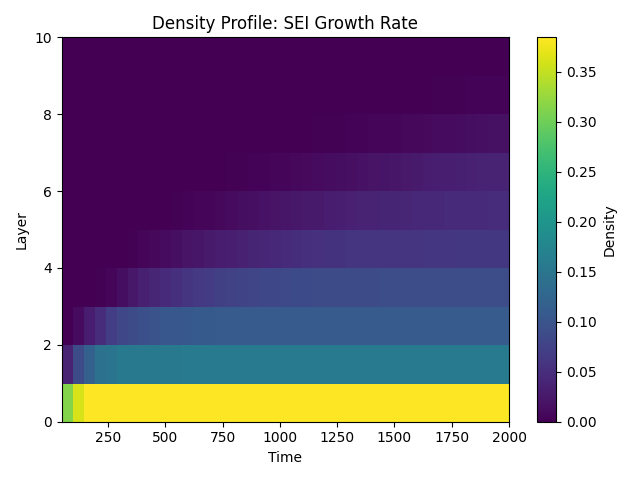
\includegraphics[scale=0.2]{figs/point_density_profile_sei_growth_rate.png}
         \caption{提高SEI生长速率}
       
     \end{subfigure}
     \hfill
     % 第三张图,这里假设你有另外三张图,分别替换图片路径和标题
     \begin{subfigure}[b]{0.19\textwidth}
         \centering
         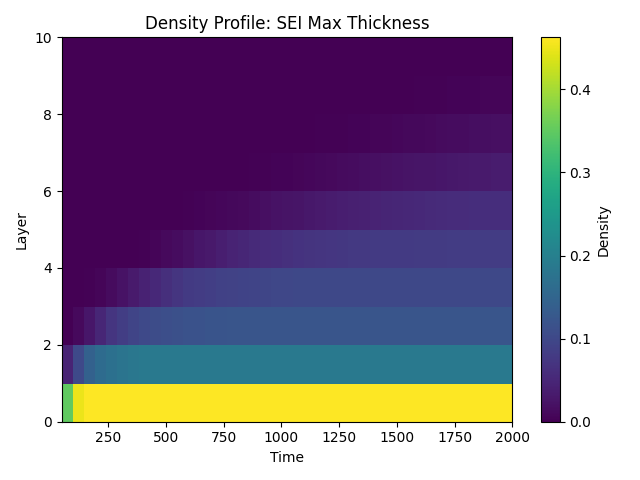
\includegraphics[scale=0.2]{figs/point_density_profile_sei_max_thickness.png}
         \caption{提高SEI最大厚度}
  
     \end{subfigure}
     \hfill
     % 第四张图
     \begin{subfigure}[b]{0.19\textwidth}
         \centering
         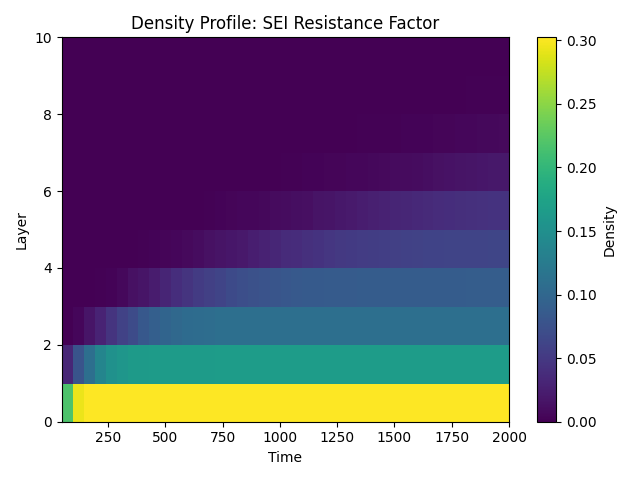
\includegraphics[scale=0.2]{figs/point_density_profile_sei_resistance_factor.png}
         \caption{提高附着概率抑制}
        
     \end{subfigure}
     \hfill
     % 第五张图
     \begin{subfigure}[b]{0.19\textwidth}
         \centering
         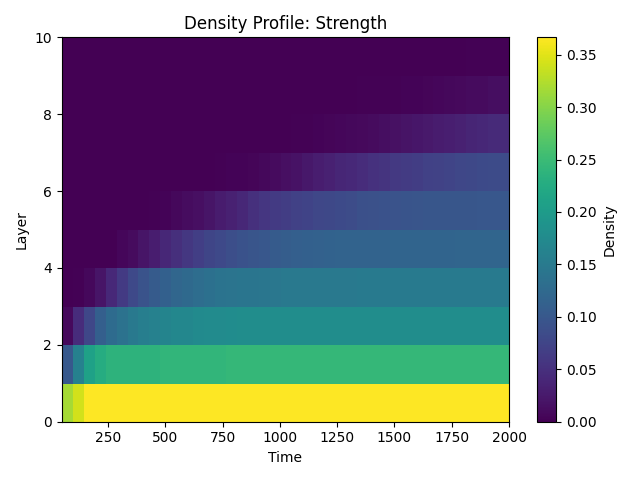
\includegraphics[scale=0.2]{figs/point_density_profile_strength.png}
         \caption{提高电场强度}
        
     \end{subfigure}
     \caption{点电极体系各层枝晶密度随时间演化}
 
 \end{figure}
 
  \begin{figure}[H]
      \centering
      % 第一张图
      \begin{subfigure}[b]{0.19\textwidth}
          \centering
          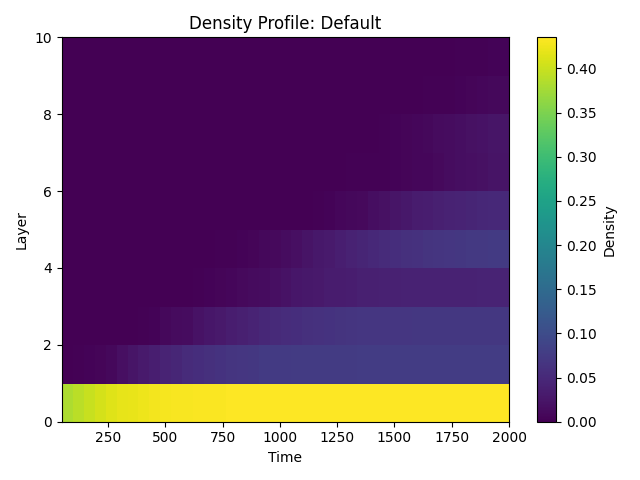
\includegraphics[scale=0.2]{figs/parallel_density_profile_default.png}
          \caption{默认参数值}
         
      \end{subfigure}
      \hfill
      % 第二张图
      \begin{subfigure}[b]{0.19\textwidth}
          \centering
          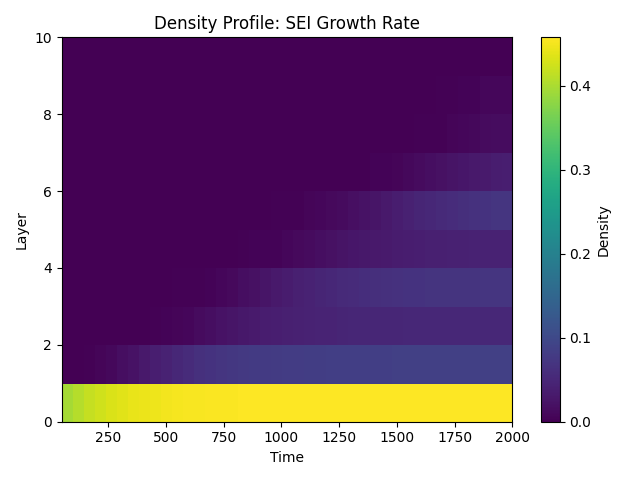
\includegraphics[scale=0.2]{figs/parallel_density_profile_sei_growth_rate.png}
          \caption{提高SEI生长速率}
        
      \end{subfigure}
      \hfill
      % 第三张图,这里假设你有另外三张图,分别替换图片路径和标题
      \begin{subfigure}[b]{0.19\textwidth}
          \centering
          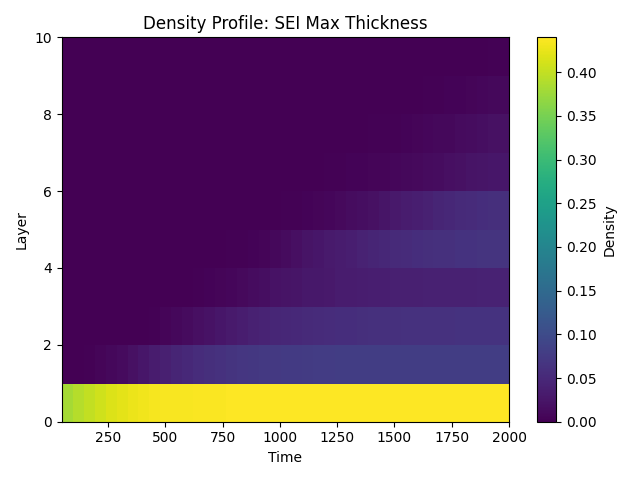
\includegraphics[scale=0.2]{figs/parallel_density_profile_sei_max_thickness.png}
          \caption{提高SEI最大厚度}
   
      \end{subfigure}
      \hfill
      % 第四张图
      \begin{subfigure}[b]{0.19\textwidth}
          \centering
          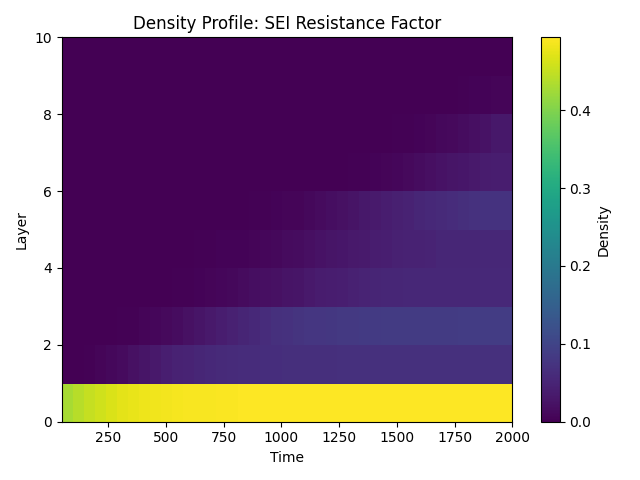
\includegraphics[scale=0.2]{figs/parallel_density_profile_sei_resistance_factor.png}
          \caption{提高附着概率抑制}
         
      \end{subfigure}
      \hfill
      % 第五张图
      \begin{subfigure}[b]{0.19\textwidth}
          \centering
          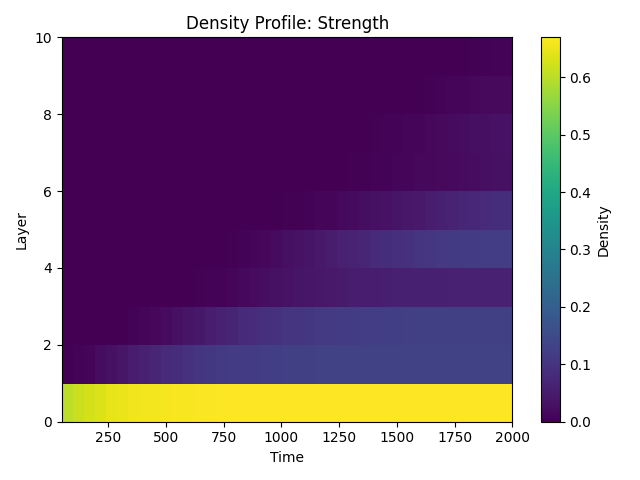
\includegraphics[scale=0.2]{figs/parallel_density_profile_strength.png}
          \caption{提高电场强度}
         
      \end{subfigure}
      \caption{平行板电极体系各层枝晶密度随时间演化}
  
  \end{figure}
  
\subsubsection{实验结果分析}
\begin{itemize}
\item \textbf{密度时空分布规律}:
在所有电极体系及参数组合下,枝晶密度均呈现显著的时空梯度特征:
\begin{itemize}
\item 空间维度:沿生长方向(底层→顶层)密度单调递减
\item 时间维度:同一空间层内,密度随沉积时间延长而增大
\end{itemize}
\item \textbf{电极构型差异}  :
平行板电极与点电极体系表现出截然不同的密度分布特性:
\begin{itemize}
    \item 平行板电极呈现\textbf{极端层间分化}:底层密度较相邻层高约3倍,且时间演化敏感性低
    \item 点电极体系层间差异较小:底层密度较相邻层高约1倍,表现出更均匀的特征
\end{itemize}

\item \textbf{电场强度效应} : 
电场强度$E$对密度分布具有全局调控作用:在两种电极体系下,提升电场强度都显著提升了各层个时间的枝晶密度

\end{itemize}

\section{结论}
本研究基于扩散限制聚集(DLA)模型,通过蒙特卡洛方法实现了锂枝晶生长的二维和三维模拟,并得出以下重要结论:

\begin{itemize}
\item \textbf{电极构型效应}:
\begin{itemize}
    \item 点电极体系产生的枝晶具有典型分形特征(分形维数$D\approx2.3$),其空间填充率显著低于平行板电极。可能是因为平行板电极线性的枝晶更容易填充空间,
    \item 平行板电极体系倾向于形成线状枝晶($D<1.0$),表现出更强的各向异性生长特性
\end{itemize}

\item \textbf{电场主导作用}:
\begin{itemize}
    \item 电场强度是影响枝晶形态的最关键参数,增强电场可使枝晶填充率提升300\%以上
    \item 枝晶累计生长速度与电场强度呈负相关。可能是因为带强电场抑制了锂离子的自由扩散,使枝晶集中在底部或中心。
\end{itemize}

\item \textbf{SEI膜调控机制}:
\begin{itemize}
    \item SEI膜参数(生长速率$\alpha$、最大厚度$d_{\text{max}}$)通过改变局部附着概率影响枝晶累计生长速率
\end{itemize}

\item \textbf{时空演化规律}:
\begin{itemize}
    \item 所有体系均呈现"底层致密-顶端稀疏"的密度梯度特征,平行板电极的空间分化更显著
    \item 生长过程存在明显的间歇停滞现象,对应实际电池中的枝晶"休眠期"
\end{itemize}
\end{itemize}

本模型为理解锂枝晶生长的微观机制提供了可视化工具,后续工作可进一步耦合热力学效应和电解液对流等物理过程。

\section{问题}
在模型构建和模拟过程中,我们遇到以下关键问题及改进方向:

\begin{itemize}
\item \textbf{模型局限性}:
\begin{itemize}
    \item 当前假设忽略了粒子间相互作用和局部浓度变化,可能导致高沉积速率下的预测偏差
    \item SEI膜演化采用经验参数化描述,缺乏第一性原理支撑
\end{itemize}



\item \textbf{实验验证不足}:
\begin{itemize}
    \item 现有结果与微观表征数据(如SEM、AFM)的定量对比仍需加强
    \item 需要设计专门的原位观测实验进行模型验证
\end{itemize}

\end{itemize}



\bibliographystyle{ieeetr}
\bibliography{refer} 

\end{document}